\documentclass[preprint,12pt]{elsarticle}
\usepackage[utf8]{inputenc}
\usepackage[a4paper,margin=2.5cm]{geometry}
\usepackage{amsmath,amssymb,amsthm}
\usepackage{graphicx}
\usepackage{booktabs}
\usepackage{array}
\usepackage{microtype}
\usepackage{xcolor}
\usepackage{xurl}
\usepackage[colorlinks=true,linkcolor=blue!50!black,citecolor=blue!50!black,urlcolor=blue!50!black]{hyperref}
\usepackage{lineno}
\usepackage{adjustbox}
\usepackage{setspace}
\biboptions{numbers,sort&compress}
\journal{Computer Methods and Programs in Biomedicine}
\emergencystretch=1.5em

\newtheorem{proposition}{Proposition}
\newtheorem{theorem}{Theorem}
\theoremstyle{remark}
\newtheorem{remark}{Remark}
\theoremstyle{definition}
\newtheorem{assumption}{Assumption}
\newcommand{\Prb}{\mathbb{P}}
\newcommand{\E}{\mathbb{E}}
\newcolumntype{L}[1]{>{\raggedright\arraybackslash}p{#1}}

\begin{document}
\begin{frontmatter}
\title{Certified adaptive examination of peripheral blood smears: when information-gain stopping fails, and what can be guaranteed instead}
\author[ud]{Qudrat Ullah\corref{cor}}
\ead{qudratafridi@mailbox.unideb.hu}
\author[ud]{Bal\'azs Harangi}
\cortext[cor]{Corresponding author.}
\affiliation[ud]{organization={Faculty of Informatics, University of Debrecen},
                 addressline={Kassai út 26}, postcode={4028}, city={Debrecen}, country={Hungary}}

\begin{abstract}
\noindent\textbf{Background and Objective:} Automated smear examination increasingly decides which fields to inspect and when to stop. We asked what such a procedure can guarantee about unexamined material, and how many expert-verified cells are needed to certify whether the blast percentage exceeds a diagnostic threshold.

\noindent\textbf{Methods:} We reimplemented the information-saturation halting rule of InfoDPP-PAC and compared it at matched cost with uniform sampling, a fixed order and confidence-based stopping on pre-registered composite specimens built from 28,280 expert-labelled cells with controlled rarity. We derived the minimax number of fields needed to certify the absence of rare evidence. For 10\% and 20\% blast thresholds we evaluated design-based, anytime-valid sequential tests with uniform and classifier-driven sampling, and tested their assumptions under acquisition shift on two external datasets, spatial clustering, unequal field sizes and reader disagreement in annotated bone-marrow regions. Analyses used exact binomial, McNemar and Wilcoxon tests and bootstrap intervals.

\noindent\textbf{Results:} The saturation rule's stopping point barely changed with rarity; with one critical field among 200 ten-cell fields it missed 76\% of positive specimens (matched uniform sampling: 85\%). Without location information, any strategy must examine 95\% of the fields to certify absence at a 5\% error level. Design-based threshold tests stayed valid wherever their assumptions held; their cost depended mainly on the margin, and within 0.02 of the threshold a 200-cell count was wrong in 11--27\% of specimens, whereas valid procedures were mostly undetermined. Against uniform sampling with the ALPHA test, classifier-driven sampling needed 0.45--0.75 times the verified cells in distribution but, at margins of 0.05--0.10, 1.3--3.0 times under two acquisition shifts that cut blast sensitivity (at 0.95 specificity) from 0.91 to 0.63 and 0.34; a 50\% uniform mixture needed 0.61--0.81 and at most 1.15 times (exploratory). Treating cells of sampled fields as independent draws exceeded the nominal error in 27 of 75 real specimens, and single-reader verification certified that reader's count, not the consensus.

\noindent\textbf{Conclusions:} Information saturation does not certify unexamined material. A classifier can reduce verification effort in distribution and increase it under shift; validity depends on the sampling design, the unit of analysis and its weighting, and the reliability of verification.
\end{abstract}

\begin{keyword}
adaptive sampling \sep sequential testing \sep anytime-valid inference \sep risk-limiting audit \sep blood smear \sep blast percentage
\end{keyword}
\end{frontmatter}

\doublespacing
\linenumbers

\section{Introduction}
A peripheral blood smear contains far more cells than any examiner inspects; a manual differential counts 100 or 200 leukocytes, with well-known sampling variability \cite{rumke1978}. Automated systems add a degree of freedom: they choose which fields to examine and when to stop. For decisions that hinge on rare cells, such as whether the blast percentage exceeds a classification threshold \cite{khoury2022who,arber2022icc}, what matters is not classifier accuracy on the examined fields but what can be said about the fields that were not examined.

Stopping rules based on \emph{information saturation} answer this question implicitly: they stop when further fields would add little information about the selector's representation of the specimen. InfoDPP-PAC \cite{mittal2026infodpp}, a recent preprint for whole-slide histopathology, selects patches greedily under a blended information-gain and relevance objective and stops when the largest remaining information gain falls below a concentration-corrected threshold; its authors state that the certificate bounds residual information in the selection objective, not diagnostic performance. That distinction is our starting point.

Risk-limiting audits bound the probability of confirming a false assertion about ballots \cite{lindeman2012gentle}; ALPHA \cite{stark2023alpha} turns assertions into bounded-mean tests for sampling without replacement, building on anytime-valid confidence sequences for that setting \cite{waudbysmith2020wor,waudbysmith2024betting,ville1939}, and Shekhar et al.\ \cite{shekhar2023rlfa} extended them to weighted, adaptive sampling with side information. Two failure modes we examine, analysing the cells of sampled fields as independent draws and averaging proportions over fields of unequal size, are the design effect and the ratio-estimation bias of cluster sampling \cite{kish1965,cochran1977}; how large they are on real smear data, and whether the tests' assumptions hold there, is not known.

We address four research questions. RQ1: does information-saturation stopping fail systematically when decision-changing evidence is rare? RQ2: why does certifying the \emph{absence} of rare evidence require near-exhaustive examination? RQ3: how many cells must be examined to certify a threshold decision under adaptive sampling? RQ4: where do the assumptions of anytime-valid audit methods break on real data? The study is methodological: most specimens are composites of real single-cell images, and no result establishes clinical diagnostic validity.

\section{Methods}
\subsection{Setting and estimands}
A specimen has $N$ fields; field $i$ holds $m_i$ cells, $B_i$ of them blasts, $M=\sum_im_i$, and $p=\sum_iB_i/M$. We distinguish \emph{detection} (has a critical field, one with at least one blast, been examined?), \emph{estimation} of $p$, and \emph{threshold certification} (is $p>\theta$?). We use $\theta=0.10$, at which the International Consensus Classification separates myelodysplastic syndrome with excess blasts from MDS/AML \cite{arber2022icc}, and $\theta=0.20$, the WHO 5th-edition threshold for acute myeloid leukaemia without defining genetic abnormalities \cite{khoury2022who}. Both count blast equivalents, which our labels do not; the thresholds are analysed separately and are inputs, not validated here. An examiner selects fields sequentially, possibly using features $x$ and past labels; a selected field is \emph{verified}, revealing its cells' labels. All probabilities are over the examiner's randomisation for a fixed specimen, so every guarantee is finite-population and design-based. It concerns the sampling frame, the fields the imaging system can present; which cells an analyser images and how the smear relates to the patient's blood are outside it.

\subsection{Certifying the absence of rare evidence (RQ2)}
Let $C$ be the set of $k$ critical fields, $M_n$ the event that none of them is among $n$ examined fields, and $h(N,k,n)=\binom{N-k}{n}/\binom{N}{n}$.
\begin{proposition}[Uniform sampling]\label{prop:uniform}
Under simple random sampling of $n$ fields without replacement, $\Prb(M_n\mid C)=h(N,k,n)$. For $k=1$ this equals $1-n/N$, so $\Prb(M_n)\le\alpha$ if and only if $n\ge\lceil(1-\alpha)N\rceil$. For every $0\le n\le N$, $[\max\{0,1-n/(N-k+1)\}]^k\le h\le(1-n/N)^k$, so $n\ge N(1-\alpha^{1/k})$ suffices.
\end{proposition}
\begin{assumption}[No location information]\label{ass:A}
The class of specimens regarded as possible, given the observed features $x$, contains every placement $C$ with $|C|=k$.
\end{assumption}
\begin{theorem}[Minimax lower bound]\label{thm:minimax}
Under Assumption~\ref{ass:A}, every policy, adaptive or not, randomised or not, that examines at most $n$ fields satisfies $\max_{|C|=k}\Prb_\pi(M_n\mid x,C)\ge h(N,k,n)$. Uniform sampling attains the bound, and every deterministic policy has worst-case miss probability 1 if $n\le N-k$.
\end{theorem}
The proof (Supplementary Section S4) applies Yao's principle \cite{yao1977}. If $k$ is unknown the worst case is $k=1$, so certifying absence at level $\alpha$ needs $\lceil(1-\alpha)N\rceil$ fields. The theorem also bears on RQ1: a rule whose halting depends only on the features and its own randomisation, not on verified labels, examines a number of fields fixed before any evidence is seen, so with one critical field its worst-case miss probability is at least $1-\bar n/N$ when it examines $\bar n$ fields on average. Informative features can beat this bound on average, through a model of where evidence lies:
\begin{proposition}[Ranked search]\label{prop:bridge}
Let one field be critical with score $S_c\sim F_1$, and let the other $N-1$ scores be independent with distribution $F_0$. A scan of the $n$ highest-scoring fields misses the critical field with probability $\E_{S_c}[\Prb(\mathrm{Bin}(N-1,1-F_0(S_c))\ge n)]$, which tends to $1-\mathrm{TPR}(t_r)$ as $N\to\infty$ with $n/(N-1)\to r$, where $t_r$ is the threshold with false-positive rate $r$ and $F_0$ is continuous and strictly increasing at $t_r$.
\end{proposition}
Certifying absence by ranking needs a sensitivity of about $1-\alpha$ at a false-positive rate of $n/N$, a property of the model, not of the design. The result is an average under independence; a ranked scan misses with certainty a critical field placed among low-scoring fields. All statements were verified exactly (Supplementary Section S1.2).

\subsection{Certifying a threshold assertion (RQ3)}
Making ``$p>\theta$'' true requires more than $\theta M$ blasts, which cannot hide in one field, so Theorem~\ref{thm:minimax} does not apply. With equal field sizes and the assorter $a_j=b_j/(2\theta)$, where $b_j$ is the blast fraction of the $j$-th sampled field, the specimen mean of $a$ exceeds $1/2$ if and only if $p>\theta$, a one-sided bounded-mean assertion. Under uniform sampling of fields, ALPHA \cite{stark2023alpha} gives a test supermartingale; rejecting when it exceeds $1/\alpha$ bounds false certification by $\alpha$ at any data-dependent stopping time. For adaptive sampling, write $p=\sum_iw_if_i$ with known weights $w_i$ and $f_i\in[0,1]$. If field $I_t$ is drawn from a predictable distribution $q_t$, the observation $Z_t=w_{I_t}f_{I_t}/q_t(I_t)$ has conditional mean equal to the unsampled mass, which under $H_0\colon p\le\theta$ is at most $\mu_t=\theta-\sum_{s<t}w_{I_s}f_{I_s}$. A betting process $\prod_s\{1+\lambda_s(Z_s-\mu_s)\}$ with predictable bets $0\le\lambda_s\le1/\mu_s$ is then a test supermartingale whatever the classifier does \cite{shekhar2023rlfa}. We used the prop-MS sampler of that work, $q_t(i)\propto w_iS_i$ with a floor, $S_i$ being the field's mean classifier score, with approximate-Kelly bets and, exploratorily, hedged bets (the average of the processes with $\lambda_s=\kappa/\mu_s$ for fixed $\kappa\in\{0.05,0.1,0.2,\dots,0.9\}$). Validity requires only known selection probabilities and verified labels; positivity of $q_t$ is needed for power and for ``$p<\theta$'' certificates, not for validity of ``$p>\theta$'', because $f_i\ge0$.

Averaging field proportions estimates $N^{-1}\sum_iB_i/m_i$, which is not $p$ when field sizes differ.
\begin{proposition}[Unequal field sizes]\label{prop:unequal}
(a) If every $m_i$ is known, $w_i=m_i/M$ and $f_i=B_i/m_i$ give $\sum_iw_if_i=p$, so the weighted test is valid for $H_0\colon p\le\theta$. (b) If only a bound $m_i\le m_{\max}$ is known, $a_i=(B_i-\theta m_i+\theta m_{\max})/m_{\max}\in[0,1]$ and $N^{-1}\sum_ia_i>\theta$ if and only if $p>\theta$, so equal-weight tests on $a_i$ with null mean $\theta$ are valid.
\end{proposition}
In (b) the margin shrinks by $\bar m/m_{\max}$, so a loose bound costs power.
\begin{remark}[Imperfect verification]\label{rem:verif}
Suppose the verifier counts the same $M$ cells as the reference and, in this specimen, its false blast calls number at most $\beta_0$ times the true non-blasts. Then $\tilde p\le p+\beta_0(1-p)$, so testing $\tilde p>\theta+\beta_0(1-\theta)$ is valid for $p>\theta$; symmetrically, testing $\tilde p<\theta(1-\beta_1)$ is valid for $p<\theta$ if missed blasts number at most $\beta_1$ times the true blasts. These are per-specimen bounds that no sampling design supplies; average disagreement rates are not such bounds, and excluding cells the reference counts can raise $\tilde p$ without any false blast call.
\end{remark}
On each specimen we compared ALPHA and betting with uniform sampling, betting with classifier-driven sampling (with and without a control variate), an invalid \emph{uncorrected} design that ranks fields by score but analyses them as uniform draws, and conventional 100- and 200-cell counts. Uniform ALPHA, the best valid design without a classifier in our runs, is the reference for cost ratios.

\subsection{Data}
KU-Optofil \cite{yarikan2026kuoptofil}: Sysmex DI-60 images of May--Gr\"unwald--Giemsa-stained peripheral blood smears labelled by haematologists; we used 28,280 cells from 275 identified patients (13 classes) in five patient-grouped folds, with 489 blasts from only 11 patients. RV-PBS \cite{rvpbs2024}: 752 annotated cells (153 blasts) from phone-camera fields, an acquisition-shift probe. MLL23 \cite{shetabboushehri2025mll23}: peripheral-blood cells (Pappenheim stain, Metafer scanner) without patient identifiers; after excluding atypical promyelocytes (blast equivalents our labels do not count), smudge cells and normoblasts, 36,529 cells including 8,606 myeloblasts. BoneMarrowWSI \cite{hofener2025bmwsi,hofener2025descriptor}: pediatric bone-marrow aspirate slides with 228 exhaustively annotated regions of about 225\,$\mu$m; we used the annotations, each reading round's labels and the region pixels.

\subsection{Representation, teachers and specimens}
Cells were embedded with a frozen DINOv2 ViT-S/14 encoder \cite{oquab2023dinov2}; a logistic probe cross-fitted by patient fold reached an out-of-fold area under the ROC curve (AUC) of 0.979 and a blast sensitivity of 0.906 at 95\% specificity. The pre-registered \emph{cell-level teacher} scores a field by its largest cell score; an exploratory \emph{field-level teacher} is a logistic regression on the pooled field embedding that the selector sees. Part~I composites have $N=200$ fields of $m\in\{1,5,10,20\}$ cells (mean-pooled embeddings) and $k\in\{1,2,5,10,20\}$ critical fields of one blast each; Part~III composites have 100 fields of 5 cells ($M=500$) with $p$ fixed exactly, and exploratory extensions use $M$ up to 4,000 and field sizes drawn from BoneMarrowWSI.

\subsection{InfoDPP-PAC and baselines (RQ1)}
No code has been released for InfoDPP-PAC, so ours is a reimplementation, not a reproduction of the authors' configuration or PAC guarantee: its objective, greedy blended gain and halting rule (Eqs.~3--7 of \cite{mittal2026infodpp}) with the published weights, the unreported constant $\rho=1$, and a halting threshold calibrated on blast-free specimens of other folds to a median stop at 16.3\% of the fields. The original runs stopped at 16.3\% of a 300-patch budget, about 2.4\% of a slide, so this setting favours InfoDPP-PAC; a 2.4\% run is also reported. A 5-field random seed fits the Gaussian process and is not counted as examined. Baselines were uniform sampling of the same size in the same specimen, a fixed field order, confidence-based stopping (at the first field with relevance $\ge0.9$, or after 30 consecutive fields $\le0.1$; illustrative thresholds, not cost-matched) and exhaustive examination (Supplementary Sections S1.4--S1.5).

\subsection{Conditions for RQ4}
The assumptions were stressed in the eight conditions of Table~\ref{tab:bench}. In the two real-data conditions each BoneMarrowWSI patient is a specimen with $4\times4$ subregions of about 56\,$\mu$m as fields, tested at its own blast proportion $\theta_s=p_s$ (an exact null at which every certification is false), with the consensus or a single reader as verifier.

\subsection{Pre-registration and statistical analysis}
Hypotheses, decision rules, seeds and scripts were frozen in five git tags before the corresponding data were generated (Supplementary Section S5); ``confirmatory'' means fresh Monte Carlo draws on a disjoint seed family, and only the external-shift and real-clustering hypotheses used data not analysed before. Later analyses, including a rerun of all cost comparisons on the same specimens for the three cell sources (seed family 20261101), are exploratory. Episodes resample cells from one pool of 275 patients, blasts from 11, so they are not independent at the patient level: exact McNemar tests on paired episodes measure Monte Carlo precision only, and miss-rate differences are reported with $t$ intervals on the five patient-grouped folds. Validity claims rest on design-based theorems that hold for every specimen; miss rates and costs are estimates for this pool. False-certification rates were tested against 0.05 with one-sided exact binomial tests (Clopper--Pearson intervals), costs with paired Wilcoxon tests (Holm correction) and ratios of medians with bootstrap intervals; real-data analyses bootstrap over patients. $\alpha=0.05$ unless stated. The implementation was checked against the reference implementation of ALPHA and with deterministic tests, including adversarial samplers and negative controls (Supplementary Section S1.4).

\section{Results}
\subsection{Information-saturation stopping (RQ1)}\label{sec:partI}
In 24,000 confirmatory episodes the median stop was 32--33 of 200 fields in every cell and varied by at most one field across rarity levels, an empirical finding: the halting statistic has no relevance term but depends on the embeddings. The information-gain term separated critical from non-critical fields with an AUC falling from 0.778 at $m=1$ to 0.525 at $m=20$, whereas a field-level teacher on the same pooled embeddings kept 0.978 to 0.827 (Fig.~\ref{fig:partI}b): the evidence survived pooling, but the halting signal did not use it.

With one critical field, InfoDPP-PAC missed it in 0.315, 0.681, 0.759 and 0.805 of specimens at $m=1$, 5, 10 and 20, against 0.82--0.85 for uniform sampling of the same size, which matched $1-n/N$ (Fig.~\ref{fig:partI}a). The advantage shrank with dilution for every $k$, but the pre-registered claim of no advantage at $m\ge10$ was not supported: the difference was $-0.087$ at $m=10$ (fold-level interval $[-0.153,-0.021]$; pre-registered episode-level interval $[-0.107,-0.067]$) and $-0.023$ $[-0.050,0.003]$ at $m=20$. Dilution, not rarity, governed the gap; rarity drove every method's absolute miss rate. Two other saturation rules missed within 0.04 of InfoDPP-PAC in every cell; a scan ranked by the field-level teacher missed 0.05--0.37, within 0.02 of Proposition~\ref{prop:bridge}. At about 2.4\% of the specimen, InfoDPP-PAC made 4--5 selections after its seed, and its advantage was $-0.17$ $[-0.27,-0.08]$ with single-cell fields and at most about 0.03 otherwise.

On real image tiles (exploratory; 3,040 tiles of about 56\,$\mu$m from 99 patients; specimens of 16--32 tiles), InfoDPP-PAC stopped after 5.4 tiles on average. In the 24 specimens with at most a quarter of the tiles critical, it missed every critical tile in 0.80 of runs against 0.70 for uniform sampling of the same size ($+0.105$ $[0.002,0.203]$), and in at least 95\% of runs in 15 specimens, as Theorem~\ref{thm:minimax} predicts for a nearly deterministic selector.

\begin{figure}[!htbp]
\centering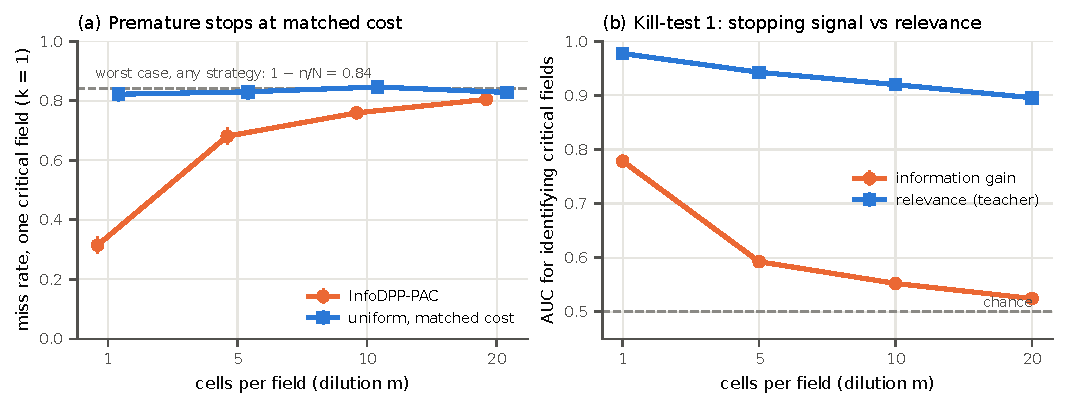
\includegraphics[width=\linewidth]{figures/fig1_partI.pdf}
\caption{Information-saturation stopping (RQ1), confirmatory run. (a) Miss rate with one critical field for InfoDPP-PAC and for uniform sampling of the same size (95\% Wilson intervals); dashed: the worst-case bound $1-n/N$. (b) AUC of the information-gain term that drives stopping and of the cell-level teacher for ranking critical above non-critical fields; dashed: the field-level teacher on the same pooled embeddings as the selector (exploratory, 10,000 separate episodes).}\label{fig:partI}
\end{figure}

\subsection{Certifying absence (RQ2)}
Figure~\ref{fig:partII} shows the fraction of fields to examine. With one critical field and $\alpha=0.05$ it is 95\% of the specimen for every $N$; with $k=10$ critical fields it is still about a quarter.

\begin{figure}[!htbp]
\centering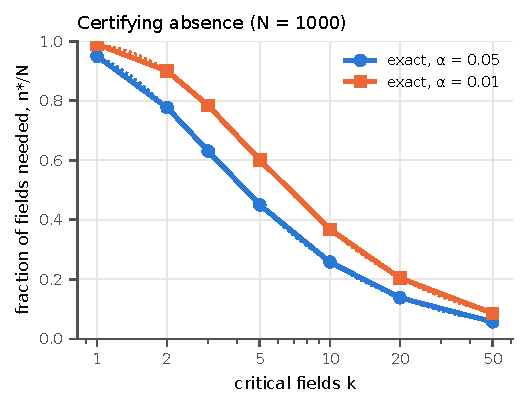
\includegraphics[width=0.6\linewidth]{figures/fig2_partII.pdf}
\caption{Certifying absence (RQ2). Fraction of fields $n^*/N$ that any strategy without location information must examine to certify the absence of $k$ critical fields ($N=1000$). Solid: exact values; dotted: the sufficient closed form $1-\alpha^{1/k}$.}\label{fig:partII}
\end{figure}

\subsection{Certified threshold decisions (RQ3)}\label{sec:rq3}
In 12,000 confirmatory 500-cell specimens, the four valid designs kept false certification at $p=\theta$ between 0.001 and 0.022, whereas the uncorrected design certified falsely in 0.993 ($\theta=0.10$) and 0.889 ($\theta=0.20$) of boundary specimens (Fig.~\ref{fig:partIII}a). Classifier-driven betting needed fewer cells than uniform ALPHA at every $p>\theta$ (all Holm-adjusted $p<10^{-59}$): 0.45--0.75 times as many, for example 75 against 165 at $p=0.15$, $\theta=0.10$; cost fell with the margin $|p-\theta|$ (Fig.~\ref{fig:partIII}b,c). Uniform betting with approximate-Kelly bets needed 1.03--1.83 times the cells of ALPHA, so savings measured against it (0.28--0.73) are overstated; with hedged bets (exploratory, 4,400 specimens) it matched ALPHA (0.98--1.17) while classifier-driven medians changed by at most 14\%.

With specimens of up to 4,000 cells (exploratory; 17,600 specimens), false certification stayed at most 0.040 at $\alpha=0.05$ and 0.007 at $\alpha=0.01$. Cost was governed mainly by the margin (Table~\ref{tab:mscale}): at margins of 0.05 or more it changed by at most 40\% between 1,000 and 4,000 cells and, with uniform sampling at $M=4{,}000$, was within 20\% of Wald's approximation $\log(1/\alpha)/\mathrm{KL}(p\,\|\,\theta)$ \cite{wald1945}; within 0.02 of the threshold it still grew with $M$, to 1,583 ($\theta=0.10$) and 2,033 cells ($\theta=0.20$) at $M=4{,}000$. The near-census at $M=500$ was a small-specimen effect.

At fixed budgets (exploratory; 2,000-cell specimens; Table~\ref{tab:decision}), within 0.02 of the threshold a 200-cell count, the usual peripheral-blood differential, was wrong in 11--27\% of specimens (100 cells: 18--37\%). Valid procedures were wrong in at most 0.7\% of specimens off the threshold but returned ``undetermined'' in 61--98\% at those margins with up to 500 cells. With a budget fixed in advance and uniform sampling, a fixed-$n$ test is decisive more often; anytime validity pays when the examiner stops on the data or samples adaptively.

\begin{figure}[!htbp]
\centering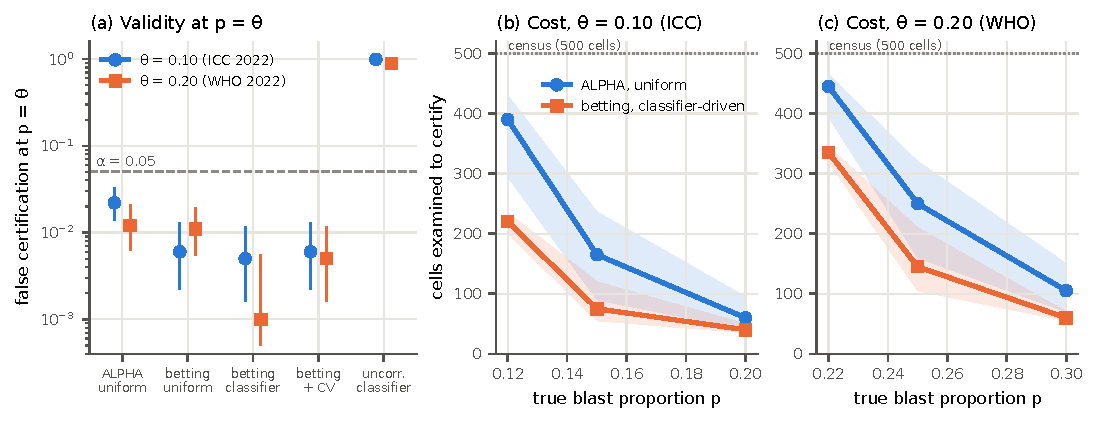
\includegraphics[width=\linewidth]{figures/fig3_partIII.pdf}
\caption{Certified threshold decisions (RQ3), confirmatory run (500-cell specimens, $\alpha=0.05$, designs paired on the same specimen). (a) False certification at $p=\theta$ with 95\% Clopper--Pearson intervals (log scale); CV: control variate; the uncorrected design analyses classifier-ranked fields as uniform draws. (b, c) Median cells to certification with interquartile bands; specimens that never certify count as 500 cells.}\label{fig:partIII}
\end{figure}

\begin{table}[!htbp]
\centering\small
\caption{Median cells to certify $p>\theta$ against specimen size $M$ (exploratory; $\alpha=0.05$; 400 specimens per cell; 5 cells per field). U: ALPHA with uniform sampling; C: betting with classifier-driven sampling; Approx.: $\log(1/\alpha)/\mathrm{KL}(p\|\theta)$. $^\dagger$Blast images reused, which affects only C. The $M=500$ column is a separate run from the confirmatory one in Fig.~\ref{fig:partIII}, so its medians differ by up to 10 cells.}\label{tab:mscale}
\begin{tabular}{@{}llrrrrrrrrr@{}}
\toprule
 & & \multicolumn{2}{c}{$M=500$} & \multicolumn{2}{c}{$M=1{,}000$} & \multicolumn{2}{c}{$M=2{,}000$} & \multicolumn{2}{c}{$M=4{,}000$} & \\
$\theta$ & $p$ & U & C & U & C & U & C & U & C & Approx.\\
\midrule
0.10 & 0.12 & 390 & 220 & 655 & 420 & 1,040 & 660 & 1,583 & 798 & 1,425\\
0.10 & 0.15 & 165 & 80 & 205 & 80 & 220 & 85 & 245$^\dagger$ & 85$^\dagger$ & 245\\
0.10 & 0.20 & 65 & 40 & 68 & 40 & 65 & 40 & 75$^\dagger$ & 40$^\dagger$ & 67\\
0.20 & 0.22 & 435 & 335 & 810 & 660 & 1,338 & 1,300 & 2,033$^\dagger$ & 2,043$^\dagger$ & 2,455\\
0.20 & 0.25 & 250 & 145 & 303 & 175 & 338$^\dagger$ & 190$^\dagger$ & 420$^\dagger$ & 185$^\dagger$ & 406\\
0.20 & 0.30 & 100 & 60 & 115 & 65 & 120$^\dagger$ & 65$^\dagger$ & 125$^\dagger$ & 70$^\dagger$ & 106\\
\bottomrule
\end{tabular}
\end{table}

\begin{table}[!htbp]
\centering\small
\caption{Three-way decisions after $n$ individually sampled cells (exploratory; $M=2{,}000$; 2,000 specimens per row; $\alpha=0.05$). Conv.: share wrong for the conventional count. Exact: one-sided hypergeometric tests at $\alpha/2$, valid at this $n$ only. Seq.: two one-sided sequential tests at $\alpha/2$, valid at every $n$. Entries for Exact and Seq.\ are shares correct\,/\,wrong; the rest is ``undetermined''.}\label{tab:decision}
\begin{tabular}{@{}llcccccc@{}}
\toprule
 & & \multicolumn{3}{c}{$n=200$} & \multicolumn{3}{c}{$n=500$}\\
\cmidrule(lr){3-5}\cmidrule(l){6-8}
$\theta$ & $p$ & Conv. & Exact & Seq. & Conv. & Exact & Seq.\\
\midrule
0.10 & 0.08 & 0.11 & 0.10\,/\,0 & 0.06\,/\,$<$0.01 & 0.03 & 0.39\,/\,0 & 0.15\,/\,$<$0.01\\
0.10 & 0.12 & 0.22 & 0.15\,/\,$<$0.01 & 0.05\,/\,$<$0.01 & 0.06 & 0.34\,/\,0 & 0.15\,/\,$<$0.01\\
0.10 & 0.15 & 0.01 & 0.60\,/\,0 & 0.31\,/\,$<$0.01 & 0.00 & 0.96\,/\,0 & 0.86\,/\,$<$0.01\\
0.20 & 0.18 & 0.19 & 0.12\,/\,$<$0.01 & 0.04\,/\,$<$0.01 & 0.08 & 0.23\,/\,0 & 0.09\,/\,$<$0.01\\
0.20 & 0.22 & 0.27 & 0.09\,/\,$<$0.01 & 0.03\,/\,$<$0.01 & 0.12 & 0.25\,/\,$<$0.01 & 0.08\,/\,$<$0.01\\
0.20 & 0.25 & 0.05 & 0.38\,/\,$<$0.01 & 0.16\,/\,0 & 0.00 & 0.87\,/\,0 & 0.59\,/\,0\\
\bottomrule
\end{tabular}
\end{table}

\subsection{Where the assumptions break (RQ4)}\label{sec:rq4}
Table~\ref{tab:bench} summarises validity and cost across eight conditions. Where their assumptions held, design-based tests kept false certification at or below 0.034; every analysis without a design-based guarantee failed in at least one condition, often while looking acceptable in another.

\emph{Classifier error and acquisition shift.} Blast sensitivity at 95\% specificity varied from 0.39 to 1.00 across the 11 KU-Optofil blast patients; applied unchanged, it fell to 0.34 [0.25, 0.42] on RV-PBS and 0.63 [0.62, 0.64] on MLL23, while its false-positive rate barely rose (0.058 and 0.060, against 0.050). Every design stayed valid, but efficiency did not transfer (Fig.~\ref{fig:rq4}a). On the same specimens (exploratory rerun), classifier-driven sampling needed 1.30 [1.18, 1.37] and 1.46 [1.36, 1.75] times the cells of uniform ALPHA on MLL23 at $p=0.15$ and 0.20, and 1.67 [1.53, 1.75] and 3.00 [2.79, 3.33] times on RV-PBS; a 50\% uniform mixture with approximate-Kelly bets reduced the confirmatory RV-PBS excess over uniform betting (1.77 at $p=0.20$) to $+23\%$ [11, 30], missing the pre-registered bound of 20\%; with hedged bets the mixture needed 0.61--0.81 times the cells of ALPHA in distribution, 0.77--0.82 on MLL23 and 0.95--1.15 on RV-PBS (exploratory).

\emph{Clustering and the unit of analysis.} Analysing the cells of sampled fields as independent draws ignores the design effect $1+(m-1)\rho$ of cluster sampling \cite{kish1965}; under strong synthetic clustering it certified falsely in up to 0.478 of boundary specimens, whereas field-level designs stayed valid. In 116 exhaustively annotated marrow regions of 75 patients, blasts were clustered weakly (bias-corrected intraclass correlation $\rho=0.013$ [0.002, 0.028] at the quadrant scale and 0.043 [0.018, 0.067] at the $4\times4$ scale used as fields below, a design effect of about 1.2 for 5-cell fields; Fig.~\ref{fig:rq4}b); in the 32 regions with at most 30\% blasts a null-centred $4\times4$ estimate was 0.059 [0.007, 0.108] (exploratory). On the real arrangements the cell-level analysis gave 0.051 overall, yet exceeded 0.05 in 27 of 75 specimens (significantly in 21; maximum 0.335), including 7 of the 23 with at most 20\% blasts (4 significantly; maximum 0.103). The weighted test of Proposition~\ref{prop:unequal}(a) stayed at or below 0.01 in every specimen: validity is a statement about each specimen, and a pooled rate can hide failures.

\emph{Unequal field sizes.} With marrow-quadrant field sizes (interquartile range 12--29 cells), averaging field proportions, the mean-of-ratios estimator \cite{cochran1977}, certified falsely in 0.38 and 0.32 of boundary specimens with blasts placed independently of size, and in every specimen with blasts enriched in small fields; both constructions of Proposition~\ref{prop:unequal} stayed at or below 0.005.

\emph{Verifier error.} The second reader called a blast in 1.1\% [0.7, 1.7] of the first reader's counted non-blasts and a non-blast in 1.2\% [0.8, 1.6] of its blasts; 2.7\% of cells were counted by only one reader. With the first reader as verifier (83 specimens), its blast proportion differed from the consensus by a median of 0.005 (maximum 0.075). Each specimen was tested at its own consensus proportion and examined almost completely, so the sign of the reader's error decided the outcome: ``$p>\theta_s$'' was certified falsely in all 23 specimens in which the reader over-counted (0.28 of runs), ``$p<\theta_s$'' in all 52 in which it under-counted (0.63), and in at most 0.008 of runs in the 8 without error. The test certified the reader's count. Remark~\ref{rem:verif} with average disagreement rates, which are not per-specimen bounds, did not repair this (0.16 and 0.42). A margin of 0.03 sufficed for ``above'' in this sample but not for ``below''; it was selected on the same specimens and is not a validated correction.

\begin{table}[!htbp]
\centering\footnotesize
\setlength{\tabcolsep}{2.6pt}
\caption{Validity and cost across conditions (summary of stored results). Top: share of specimens in which ``$p>\theta$'' was certified at the exact null $p=\theta$ ($\alpha=0.05$; larger of $\theta=0.10$ and $0.20$ where both were run; 400--1,000 specimens). BoneMarrowWSI: rate pooled over runs with $\theta_s=p_s$, with the largest specimen rate in brackets (75 and 83 specimens, 400 orders each). Bottom: median cells to certify $p=0.15$ against $\theta=0.10$; uncertified specimens count all their cells. Specimens hold 500 cells, about 1,300 with unequal fields, and a median of 105 real cells in BoneMarrowWSI. Stressed: the assumption the condition tests (unit: analysed unit equals sampled unit; target: cell-weighted $p$). C/X: confirmatory/exploratory run. ---: not run or not applicable. $^a$With unequal fields and in BoneMarrowWSI, ALPHA uses the bounded assorter and betting the known counts (Proposition~\ref{prop:unequal}). $^b$Coincides with ALPHA for equal fields; 1.00 with blasts enriched in small fields. $^c$Exploratory rerun with all designs on the same specimens (seed family 20261101); uniform ALPHA sees only labels, so its cost does not depend on the cell source. Single reader with a margin of 0.03: 0.0003 [0.013].}\label{tab:bench}
\begin{adjustbox}{max width=\linewidth}
\begin{tabular}{@{}l cccc cc cc@{}}
\toprule
 & \multicolumn{4}{c}{Composites of KU-Optofil cells} & \multicolumn{2}{c}{External cells} & \multicolumn{2}{c}{BoneMarrowWSI}\\
\cmidrule(lr){2-5}\cmidrule(lr){6-7}\cmidrule(l){8-9}
 & In distr. & Clustered & Confusable & Unequal & RV-PBS & MLL23 & Real & One\\
 & & & backgr. & fields & & & arrangem. & reader\\
\emph{Stressed} & --- & \emph{unit} & \emph{classifier} & \emph{target} & \multicolumn{2}{c}{\emph{classifier transfer}} & \emph{geometry} & \emph{verifier}\\
\emph{Status} & C & C & X & X & C & X & X & X\\
\midrule
\multicolumn{9}{@{}l}{\emph{False certification of ``$p>\theta$'' at $p=\theta$}}\\
ALPHA, uniform$^{a}$ & 0.022 & 0.025 & 0.031 & 0 & 0.026$^c$ & 0.034$^c$ & 0 [0] & ---\\
Betting, uniform$^{a}$ & 0.011 & 0.005 & 0.011 & 0.005 & 0.011 & 0.011 & 0.001 [0.010] & 0.277 [1.00]\\
Betting, classifier-driven & 0.005 & 0.003 & 0.007 & 0.001 & 0.001 & 0.001 & --- & ---\\
Betting, 50\% mixture & 0.014 & --- & --- & --- & 0.003 & 0.004 & --- & ---\\
Hedged betting, 50\% mixture$^c$ & 0.028 & --- & --- & --- & 0.025 & 0.030 & --- & ---\\
\addlinespace
Ranked, analysed as uniform & 0.993 & --- & --- & --- & --- & --- & --- & ---\\
Cells of fields as draws & 0.041 & 0.478 & --- & --- & --- & --- & 0.051 [0.335] & ---\\
Mean of field proportions$^{b}$ & --- & --- & --- & 0.379 & --- & --- & 0.062 [1.00] & ---\\
100-cell count, ``above'' & 0.427 & 0.388 & --- & --- & --- & --- & --- & ---\\
\midrule
\multicolumn{9}{@{}l}{\emph{Median cells to certify $p=0.15$ against $\theta=0.10$}}\\
ALPHA, uniform$^{a}$ & 165 & 345 & 160 & 1{,}031 & 165$^c$ & 165$^c$ & --- & ---\\
Betting, uniform$^{a}$ & 270 & 355 & 265 & 646 & 260 & 283 & --- & ---\\
Betting, classifier-driven & 75 & 55 & 105 & 297 & 265 & 215 & --- & ---\\
Betting, 50\% mixture & 145 & --- & --- & --- & 285 & 220 & --- & ---\\
Hedged betting, 50\% mixture$^c$ & 110 & --- & --- & --- & 190 & 135 & --- & ---\\
\bottomrule
\end{tabular}
\end{adjustbox}
\end{table}

\begin{figure}[!htbp]
\centering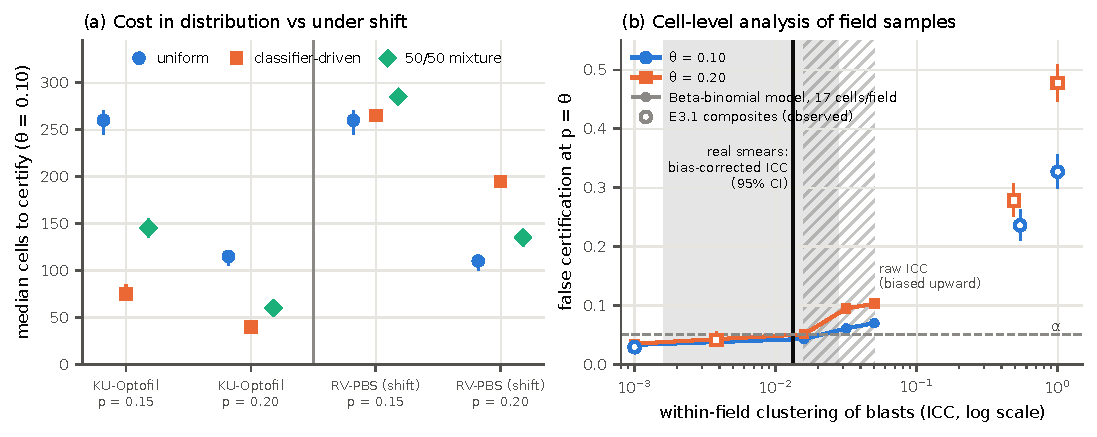
\includegraphics[width=\linewidth]{figures/fig4_rq4.pdf}
\caption{Where the assumptions break (RQ4). (a) Median cells to certify $p>0.10$ with 95\% bootstrap intervals, in distribution (KU-Optofil) and under two acquisition shifts (MLL23, RV-PBS): uniform sampling with ALPHA, classifier-driven betting, and a 50\% mixture with hedged bets, all on the same specimens (exploratory rerun, 400 specimens per point); all designs kept false certification at or below 0.034. (b) False certification at $p=\theta$ when the cells of sampled fields are analysed as individual draws: composites with scattered or clustered arrangements (open markers) and a Beta-binomial model with 17 cells per field (lines). Solid band and line: bias-corrected clustering of real marrow regions (exploratory); hatched: the raw, upward-biased estimate, for comparison.}\label{fig:rq4}
\end{figure}

\subsection{Pre-registered hypotheses}
Of the 15 pre-registered empirical hypotheses, 12 were supported, and the 5 implementation checks passed (Table~\ref{tab:hyp}). The proposal's original rarity hypothesis (Kill-test 2) had already failed on exploratory data and was replaced by H1b before the confirmatory run.

\begin{table}[!htbp]
\centering\small
\caption{Pre-registered hypotheses and verdicts. Type: E, an empirical claim; V, a check of the implementation or of a property that holds by theorem. KT2, the proposal's rarity hypothesis, was tested on exploratory data only and is not counted among the 20 pre-registered hypotheses.}\label{tab:hyp}
\begin{tabular}{@{}lllL{8.2cm}l@{}}
\toprule
RQ & ID & Type & Hypothesis (abridged) & Verdict\\
\midrule
1 & KT2 & E & Gap to uniform sampling widens as evidence becomes rarer (proposal; exploratory; replaced by H1b) & \textbf{not supported}\\
1 & H1a & E & InfoDPP-PAC stop point unchanged across rarity levels & supported\\
1 & H1b & E & Advantage over matched-cost uniform sampling shrinks with dilution & supported (4/4)\\
1 & H1c & E & No advantage ($\pm0.05$) at $m\ge10$, $k=1$ & \textbf{not supported}\\
2 & H1d & V & Uniform miss rate equals $1-n/N$ & supported\\
1 & KT1 & E & Information gain and relevance are separable signals & supported\\
3 & H3a & V & All four designs valid at both thresholds & supported\\
3 & H3b & E & Uncorrected adaptive selection invalid & supported\\
3 & H3c & E & Classifier-driven betting cheaper than uniform ALPHA & supported\\
3 & H3d & E & Cost decreases with the margin & supported\\
4 & H4a & E & Blast sensitivity drops under acquisition shift & supported\\
4 & H4b & E & False-positive rate rises under shift & \textbf{not supported}\\
4 & H4c & V & Certificate valid with shifted side information & supported\\
4 & H5a & V & Field-level tests valid under clustering & supported\\
4 & H5b & E & Cell-level analysis of field samples invalid under clustering & supported\\
4 & H5c & E & Clustering raises the cost of valid certification & supported\\
4 & H6a & V & Defensive mixture valid & supported\\
4 & H6b & E & Mixture caps loss under shift below 20\% & \textbf{not supported}\\
4 & H6c & E & Mixture keeps $\ge50\%$ of in-distribution saving & supported\\
4 & H6d & E & Cost reversal under shift replicates & supported\\
4 & H7a & E & Blasts spatially clustered in real smears & supported\\
\bottomrule
\end{tabular}
\end{table}

\section{Discussion}
\subsection{What is guaranteed, and by what}
Our results separate three quantities that are often reported together. \emph{Model confidence} about examined fields says nothing about unexamined ones. \emph{Information saturation} concerns the selector's representation; its association with decision-relevant evidence vanished once cells were pooled into fields, although the pooled representation still carried the evidence. \emph{Design-based certification} bounds the probability of a false threshold decision for the specific specimen, given known selection probabilities and verified labels. Only the third concerns what was not examined; it held in every condition we tested, specimen by specimen, whatever the classifier did. It concerns the imaged frame and the verifier's labels, not the patient (Table~\ref{tab:assump}).

\begin{table}[!htbp]
\centering\small
\caption{What each guarantee assumes, and what happened when the assumption was tested.}\label{tab:assump}
\begin{tabular}{@{}L{4.2cm}L{2.6cm}L{7.4cm}@{}}
\toprule
Assumption & Needed for & Test and result\\
\midrule
No location information & Theorem~\ref{thm:minimax} & Features informative on composites: ranking helps on average, through a model (Proposition~\ref{prop:bridge}), not for every placement\\
Selection probabilities known & Validity & Uncorrected ranking: false certification 0.89--0.99\\
Analysis unit equals sampled unit & Validity & Cells as draws (design effect ignored): up to 0.34 per real specimen, 0.33--0.48 under strong clustering\\
Target is the cell-weighted $p$ & Validity & Averaging proportions: 0.32--0.38; Proposition~\ref{prop:unequal} restores $\le0.005$\\
Verified label equals truth & Validity for the true $p$ & Single reader: false certification wherever its count lay on the claimed side (0.28 ``above'', 0.63 ``below'')\\
Accurate classifier, exchangeable errors & Efficiency only & Validity held under shift ($\le0.034$); cost relative to uniform ALPHA rose from 0.45--0.75 to 1.3--3.0 at margins of 0.05--0.10\\
\bottomrule
\end{tabular}
\end{table}

\subsection{Relation to previous work}
R\"umke's binomial analysis of manual differentials \cite{rumke1978} implies imprecision for rare cell types; at a threshold a 200-cell count was wrong in up to 27\% of our specimens. Proposition~\ref{prop:uniform} and Theorem~\ref{thm:minimax} are finite-population, design-based counterparts of the ``rule of three'' \cite{hanley1983}, extended to every strategy without location information; fixed-effort practice rules, such as examining at least 100 thick-film fields before reporting no malaria parasites \cite{who2016malariasop}, face the same worst case. Classification accuracy, the focus of work on blast recognition \cite{matek2019aml}, affected efficiency rather than validity. The failures of cell-level analysis and of averaged proportions are textbook survey-sampling results \cite{kish1965,cochran1977}, and classifier-driven sampling is probability-proportional-to-size sampling \cite{hansen1943,horvitz1952}; our experiments add their size on real smear arrangements and their consequence for anytime-valid certificates. The tests of Stark \cite{stark2023alpha} and Shekhar et al.\ \cite{shekhar2023rlfa} transferred to smear examination; active statistical inference \cite{zrnic2024active} also lets a model choose which units to label, but with fixed-sample guarantees for a superpopulation. Stratified tests \cite{spertus2024stratified} and prediction-powered inference \cite{angelopoulos2023ppi,csillag2025ppe} were not implemented.

\subsection{Practical implications}
First, certify a proportion against a stated threshold rather than the absence of rare cells, which requires a near-census. Second, record selection probabilities, analyse the unit that was sampled, and weight fields by their cell counts. Third, keep a uniform component in classifier-driven sampling, and judge savings against the best valid uniform design. Fourth, report ``undetermined'', the honest outcome of a few hundred cells near the threshold. Fifth, relating a certificate to the true proportion requires a separately established bound on verifier error.

\subsection{Limitations}
Most specimens are composites from one laboratory, and all KU-Optofil blasts come from 11 patients, so cost and miss-rate comparisons are imprecise. The spatial, tile and verifier analyses use small, mostly high-blast pediatric bone-marrow specimens, not peripheral blood, and test each specimen against its own blast proportion, not fixed diagnostic thresholds; they do not establish clinical validity. The external datasets lack patient identifiers, so their intervals understate uncertainty, and reading rounds are not identified experts. Several analyses, including every cost comparison against uniform ALPHA on external cells and all hedged-bet results, are exploratory, and the pre-registration tags are timestamped by the hosting service only. InfoDPP-PAC is a reimplementation calibrated to a cost; varying its unreported settings, or replacing it with two other saturation rules, gave the same result. We used one frozen encoder, and costs count expert-verified cells, not imaging or computing time.

\section{Conclusions}
Information saturation does not certify what remains unexamined, and without location information certifying the absence of rare evidence requires examining nearly the whole specimen. Threshold decisions about the blast proportion can instead be certified with finite-sample, anytime-valid guarantees. A classifier can reduce the cells an expert must verify in distribution and increase them under shift, so it should be combined with a uniform component; validity rests on the sampling design, the unit of analysis and weighting, and the reliability of verification. Fully annotated peripheral-blood smears and verification by identified haematologists are the most important next steps.

\section*{Ethics statement}
This study used only publicly available, de-identified datasets released under open licences (KU-Optofil, MLL23 and BoneMarrowWSI under CC BY 4.0; RV-PBS as distributed by its authors). No new data were collected from human participants and no participant was contacted, so ethical approval and informed consent were not required for this secondary analysis. [To be confirmed against the University of Debrecen's requirements.]

\section*{CRediT authorship contribution statement}
\textbf{Qudrat Ullah:} Conceptualization, Methodology, Software, Formal analysis, Investigation, Data curation, Visualization, Writing -- original draft. \textbf{Bal\'azs Harangi:} Supervision, Writing -- review \& editing.

\section*{Declaration of competing interest}
The authors declare that they have no known competing financial interests or personal relationships that could have appeared to influence the work reported in this paper.

\section*{Funding}
This research did not receive any specific grant from funding agencies in the public, commercial, or not-for-profit sectors.

\section*{Data and code availability}
All code, the pre-registration with its git history, the audit trail and the analysis outputs are available at \url{https://github.com/Afridi-7/certified-adaptive-pbs}; a release will be archived on Zenodo with a DOI. KU-Optofil, BoneMarrowWSI-PediatricLeukemia and MLL23 are public datasets under CC BY 4.0. RV-PBS is publicly distributed by its authors without a stated licence and was used for research only.

\section*{Supplementary material}
The supplementary file gives the full methods (Section S1, including the InfoDPP-PAC reimplementation and all deviations), the complete results with all sensitivity and exploratory analyses (Sections S2 and S3), the proof of Theorem~\ref{thm:minimax} (Section S4) and the pre-registration audit trail (Section S5).

\section*{Acknowledgements}
The authors thank Iqra Muhammad for her advice and support during this work.

\section*{Declaration of generative AI and AI-assisted technologies in the manuscript preparation process}
The research questions and study design come from the first author's research proposal. During the preparation of this work the authors used Claude (Anthropic) as an assistant for coding, checking calculations and references, and editing the text. The authors reviewed and edited all output and take full responsibility for the content of the published article.

\bibliographystyle{elsarticle-num}
\bibliography{refs}

\end{document}
